\documentclass[11pt,a4paper]{report}

\usepackage[english]{babel} 
\usepackage[utf8]{inputenc} % Unicode
\usepackage{graphicx} 
\usepackage{url} 
\usepackage{amsmath}
\usepackage{textcomp} 
\usepackage{multirow} 
\usepackage[pdftex,hidelinks]{hyperref}
\usepackage{listings}
\usepackage{natbib}
\usepackage{graphicx}
\usepackage{hyperref}
\usepackage{verbatim}
\usepackage{textcomp}
\usepackage{caption}
\usepackage{subcaption}
\usepackage{acronym}

\def\R{{\textsl{R }}}
\def\Shiny{\textsl{Shiny }}
\def\sar{\textsl{SARS-CoV-2 }}



\title{Development of a \Shiny application to visualize SARS-CoV-2 vaccination data of Portugal}

\author{
  Bruna Araújo\\
  \texttt{A84408}
  \and
  Matias Capitão\\
  \texttt{A82726} \\ 
  \\ Mentoring:\\
  Cecília Castro\\
  \and
  Rafael Antunes\\
  \texttt{A77457}
}
\date{May or June 2021}



\begin{document}

\maketitle

\begin{abstract}
% Apagar daqui
    ************* Ao fim retornamos aqui.\\ Entretanto encontrei isto para nos ajudar a fazer o Abstract *************\\ \\
%até aqui
    Write the abstract at the very end, when you’ve completed the rest of the text. There are four things you need to include:\\ \\

    Your research problem and objectives\\
    Your methods\\
    Your key results or arguments\\
    Your conclusion

\end{abstract}

\tableofcontents
\newpage

\listoffigures
\newpage

\listoftables
\newpage

{\huge\textbf{Acronym List}}\\
\begin{acronym}[MPC] % Give the longest label here so that the list is nicely aligned
\acro{IDE}{Integrated Development Environment}
\acro{WHO}{World Healh Organization}
\acro{EU}{European Union}
\acro{ECDC}{European Centre for Disease Prevention and Control}

\end{acronym}


\chapter{Introduction}
\section{\R and \Shiny}

\textbf{\R}  is a program created in 1993 by Ross Ihaka and Robert Gentleman  defined as
"a language and environment for statistical computing and graphics" \cite{R-project website}.
\\
 RStudio is an integrated development environment (IDE) for R. \cite{rstudio}
\begin{figure}
\centering
\begin{subfigure}{.5\textwidth}
  \centering
  
\includegraphics[width=3cm]{images/R.jpg}
  \label{fig:sub1}
\end{subfigure}%
\begin{subfigure}{.5\textwidth}
  \centering
  
\includegraphics[width=5cm]{images/Rstudio.png}
  \label{fig:sub2}
\end{subfigure}
\caption{Logos of R and RStudio}
\label{fig:test}
\end{figure}
\\
R has over 10,000 packages in the CRAN repository which are constantly growing. 
\textbf{\Shiny} is an \R package that makes easy to build interactive web applications \cite{shiny} .
\\
With this package we can combine the computational power of \R with the versatility and interactivity of modern web. This feature it's relevant to develop plots and graphics that can be understood by everyone, and looking pretty while doing it.




\section{SARS-CoV-2}
\subsection{Brief description}



\sar is the name of the coronavirus that caused the current COVID-19 pandemic. According to \ac{WHO}, the first human cases of COVID-19, were first reported from Wuhan City, China, in December 2019. 
The main symptoms of Covid-19 are fever, cough, breathing difficulties, loss of smell and taste. 
It's a disease that attacks all age levels and is transmitted mainly by air, via particles that we expel. \\
There are several reasons for the pandemic to spread globally, mainly the fact that a patient may be asymptomatic, which can cause him to transmit the virus without knowing it. For the same reason, the fact that the incubation period is about 14 days is also a factor to be taken into account. 

\subsection{Vaccination}
Vaccines are substances made up of pathogens (viruses or bacteria), living or dead, or their derivatives. They stimulate the immune system to produce antibodies that act against pathogens that cause infections.

Vaccination is a way to protect people from harmful diseases. It uses the body's natural defenses to build resistance to specific infections and makes the
 stronger immune system.
It reduces the possibility of contracting the disease and thus prevents it from spreading.
\\
As soon as the COVID-19 pandemic took hold in the world, research for the production of safe and effective vaccines began immediately. Vaccination is critical to ending the COVID-19 pandemic. WHO is working tirelessly with partners to develop, manufacture and distribute safe and effective vaccines.
\\
Until May 10, 13 vaccines have been authorized by at least one national regulatory authority for public use. However, in Europe, after consulting the list of authorized vaccines on the \cite {EU} official website of the \ac{EU}, we have four vaccines available: 
\begin{itemize}
    \item BioNTech-Pfizer - (2020/12/21)
    \item Moderna - (2021/01/06)
    \item AstraZeneca - (2021/01/29)
    \item Johnson \& Johnson - (2021/03/11)
\end{itemize}
But it's not the vaccines that will stop the pandemic, it's the vaccination. 
\\





\section{Portugal}

\subsection{Brief description}
Portugal is a country in Europe with a resident population of around 10.2 million inhabitants.  \\
According to the local statistics institute, INE (Instituto Nacional de Estatística - National Statistics Institute), in the publication dated 2019 and edited in 2020, called \cite{pubINE}"Demographic Statistics - 2019", we can find some interesting information such as:
\begin{itemize}
    \item In percentage terms, relative to \textbf{sex},
    \begin{itemize}
        \item \textbf{47,2\textdiscount} of the population is \textbf{male};
        \item \textbf{52,8 \textdiscount} of the population is \textbf{female}.
    \end{itemize}  
    \item In terms of \textbf{age} percentages, 
    \begin{itemize}
        \item \textbf{13,6\textdiscount} of \textbf{young people} (0-14 y/o);
        \item \textbf{64.3\textdiscount} of people of \textbf{working age} (15-64 y/o);
        \item \textbf{22.1\textdiscount} of \textbf{elderly people} (65+ y/o). 
    \end{itemize}
\end{itemize}

Se calhar por aqui alguns graficos relativos ao descrito acima nao é má ideia.

\subsection{Regions}
In terms of NUTS II regions, Portugal is divided in seven groups.
The structuring of the Portuguese territory according to the New Territorial Units for Statistical Purposes, NUTS 2013,  in application in the National Statistical System since 1 January 2015 is composed of seven NUTS II: North, Centre, Lisbon Metropolitan Area (AML), Alentejo and Algarve regions, on the mainland, and the two autonomous regions. \cite{INEE}
\begin{figure}[h]
\centering % para centralizarmos a figura
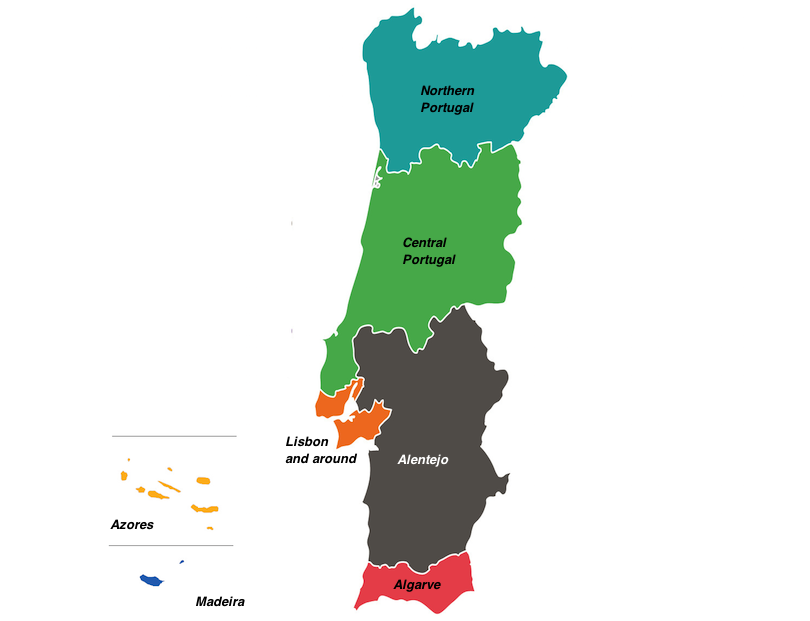
\includegraphics[width=10cm]{images/portugal.png} 

\caption{Portugal's Regions}
\label{figura:qualquernome}
\end{figure}

We'll describing them below, also mentioning some statistical data that may be interesting. \\
All information related to the labor market in the regions was obtained by consulting the  website of the European Commission \cite{trab}. The demographic percentages presented are based on data from  National Institute of Statistics of Portugal, INE. 

\subsubsection{North}
The employment structure in the North region presents 3 sub-regions with specific characteristics: 
The Porto Metropolitan Area, with a strong incidence of services (mainly trade) with greater technological and knowledge intensity. A surrounding shore, where industrial employment is  higher than the national average and rural areas, where nearly half of employment is concentrated in agriculture or non-commercial services.

In terms of {\textbf{demographics}}:
    \begin{itemize}
        \item Population density: {34,73\textdiscount} . 
        \item Gender: {47,2\textdiscount} male and {52,8\textdiscount} female.
        \item Age: 
        \begin{itemize}
        \item {12,63 \textdiscount} aged 14 and younger;
        \item {66,43\textdiscount} aged 15 to 64;
        \item {20,94\textdiscount} aged 65 and older.
        \end{itemize}
    \end{itemize}

\subsubsection{Center}
In this region, the Services sector is the most relevant in terms of employment - with emphasis on Trade and Vehicle Repair, Health and Social Support Services and the Education. \\
In terms of {\textbf{demographics}}:
    \begin{itemize}
        \item Population density: {21,54\textdiscount} . 
        \item Gender: {47,42\textdiscount} male and {52,58\textdiscount} female.
        \item Age: 
        \begin{itemize}
        \item {12,05 \textdiscount} aged 14 and younger;
        \item {63,42\textdiscount} aged 15 to 64;
        \item {24,53\textdiscount} aged 65 and older.
        \end{itemize}
    \end{itemize}
    
\subsubsection{Metropolitan area of Lisbon }
This is the region with the highest population density in the country. It's the region with the highest concentration of services, with emphasis on services provided mostly by the Public Sector; Education; Health and social support services.\\
In terms of {\textbf{demographics}}:
    \begin{itemize}
        \item Population density: {27,81\textdiscount} . 
        \item Gender: {46,71\textdiscount} male and {53,29\textdiscount} female.
        \item Age: 
        \begin{itemize}
        \item {15,88\textdiscount} aged 14 and younger;
        \item {62,04\textdiscount} aged 15 to 64;
        \item {22,08\textdiscount} aged 65 and older.
        \end{itemize}
    \end{itemize}
    
\subsubsection{Alentejo}
This is the region with the lowest population density in the country. Most of the region's territory is dedicated to Agriculture, allied to cattle breeding and also forestry.\\
In terms of {\textbf{demographics}}:

    \begin{itemize}
        \item Population density: {6,84\textdiscount} . 
        \item Gender: {47,97\textdiscount} male and {52,03\textdiscount} female.
        \item Age: 
        \begin{itemize}
        \item {12,4\textdiscount} aged 14 and younger;
        \item {62,05\textdiscount} aged 15 to 64;
        \item {25,55\textdiscount} aged 65 and older.
        \end{itemize}
    \end{itemize}
    
\subsubsection{Algarve}
The economic structure of this region is based on 5 strategic sectors associated with the region's natural resources: hospitality, catering and tourism, health, creative activities, agri-food and maritime activities. 
In terms of {\textbf{demographics}}:
    \begin{itemize}
        \item Population density: {34,73\textdiscount} . 
        \item Gender: {47,2\textdiscount} male and {52,8\textdiscount} female.
        \item Age: 
        \begin{itemize}
        \item {12,63\textdiscount} aged 14 and younger;
        \item {66,43\textdiscount} aged 15 to 64;
        \item {20,94\textdiscount} aged 65 and older.
        \end{itemize}
    \end{itemize}
    
\subsubsection{Azores autonomous region}
The region's economy is fundamentally based on activities mainly from the Public Sector (Public Administration, Social Security, Education, Health and Social Support activities). The activities of Trade and Repair of Vehicles and Accommodation and Restoration are equally important in employment in the region. \\
In terms of {\textbf{demographics}}:
    \begin{itemize}
        \item Population density: {2,36\textdiscount} . 
        \item Gender: {48,55\textdiscount} male and {51,45\textdiscount} female.
        \item Age: 
        \begin{itemize}
        \item {15,37\textdiscount} aged 14 and younger;
        \item {69,69\textdiscount} aged 15 to 64;
        \item {14,99\textdiscount} aged 65 and older.
        \end{itemize}
    \end{itemize}
    
\subsubsection{Madeira autonomous region }
In terms of more established work areas, this region is very similar to the Azores region. Tourism has an important role for both regions.\\
In terms of {\textbf{demographics}}:
    \begin{itemize}
        \item Population density: {2,47\textdiscount} . 
        \item Gender: {46,67\textdiscount} male and {53,33\textdiscount} female.
        \item Age: 
        \begin{itemize}
        \item {13,11\textdiscount} aged 14 and younger;
        \item {69,91\textdiscount} aged 15 to 64;
        \item {16,98\textdiscount} aged 65 and older.
        \end{itemize}
    \end{itemize}









\section{SARS-CoV-2 in Portugal}

\subsection{Brief description}

%SARS-CoV-2 (Severe Acute Respiratory Syndrome coronavirus) is a new type of coronavirus that causes a respiratory disease called coronavirus disease 19, know as COVID-19. It was first detected in December 2019 has quickly spread globally.

Portugal recorded the first confirmed case of COVID-19 on March 2 and the first death occurred
on March 16. Since then we have added more than 800 thousand registered cases and more than 16 thousand deaths.

Portugal was severely affected by COVID-19, being considered, in the middle of January 2021, as the worst country in the world in terms of infection and mortality rates per million inhabitants and the worst country in Europe with the highest average of cases COVID-19 daily reports, with Portugal reaching a maximum of 16432 cases and 303 deaths on 28 January 2020.

\subsection{Vaccination}

   To end this pandemic, a large part of the world needed to be immune to the virus. The safest way to achieve this was through a vaccine, so with the help of investments by companies, governments, international health organizations and university research groups it was possible to develop a series of vaccines including Phyzer, Moderna, Astrazeneca, Johnson & Johnson, among others.

   The first vaccine administered in Portugal was on December 27, 2020. The first vaccine was António Sarmento, 65, director of the Infectious Diseases Service, at Hospital de São João, in Porto and since then more than 2 million doses of vaccine have been administered. Despite the fact that the entire Portuguese population has access to a vaccine, depending on their clear clinical condition, Portugal opted for a vaccination plan divided into 3 phases, that is, priority groups were defined, as they are more vulnerable to COVID-19, as an example health professionals, professionals and residents of residential structures for the elderly and similar institutions, who were part of the first vaccination phase.






\chapter{Application}

\section{Research}
The data that we used to develop this application was downloaded from the \ac{ECDC} which is an \ac{EU} agency aimed at strengthening Europe's defenses against infectious diseases.
\\
As we can read in the \ac{ECDC} website \cite{dataDownload}, they are providing an overview of the progress in the rollout of COVID-19 vaccines in adults across \ac{EU} countries.
\begin{figure}[h]
\centering % para centralizarmos a figura

\includegraphics[width=3cm]{images/ecdc.png} 

\caption{ECDC logo}
\label{figura:qualquernome}
\end{figure}

The data is collected through The European Surveillance System (TESSy) and they publish the updated data, every week on Thursdays. In Portugal, the entity responsible to send the data is the Ministry of Health.

\subsection{Structure of the data}
The dataset  downloaded in each interaction with the app in format \verb!csv!, has the following columns:

\begin{itemize}
    \item \textbf{YearWeekISO} - Date information in weeks:  week number and year;
    \item \textbf{FirstDose} - Number of first dose vaccine administered to individuals during the reporting week;
    \item \textbf{FirstDoseRefused} - Number of individuals refusing the first vaccine dose;
    \item \textbf{SecondDose} - Number of second dose vaccine administered to individuals during the reporting week;
    \item \textbf{UnknownDose} - Number of doses administered during the reporting week where the type of dose was not specified;
    \item \textbf{NumberDosesReceived} - Number of vaccine doses distributed by the manufacturers to the country during the reporting week;
    \item \textbf{Region} -  Region of the Reporting Country.
   
    In order to know the region to which these codes relate to, it was necessary another excel document. This document also brought another important component, namely, the population of each region. Having said this:
    \begin{itemize}
        \item PTCSR01 - Alentejo; Population - 466 690
        \item PTCSR02 - Algarve; Population - 438 406
        \item PTCSR03 - Autonomous Region of Azores ; Population - 242 796
        \item PTCSR04 - Centre; Population - 1 650 394
        \item PTCSR05 - Metropolitan Area of Lisbon; Population - 3 674 534
        \item PTCSR06 - Autonomous Region of Madeira; Population - 254 254
        \item PTCSR07 - North; Population - 3 568 835

    \end{itemize}
    \item \textbf{Population} - Age-specific population for the country (unfortunately, in Portugal, this hasn't been exactly right, it only has the total population of Portugal);
    \item \textbf{ReportingCountry} - The country that is providing the information;
    \item \textbf{TargetGroup} - Target group for vaccination;
    \item \textbf{Vaccine} - Name of vaccine;
    \item \textbf{Denominator} - Population denominators for target groups.

We will show next, a little example of the dataset already filtered for Portugal.

\end{itemize}

\begin{figure}[h]
\centering % para centralizarmos a figura
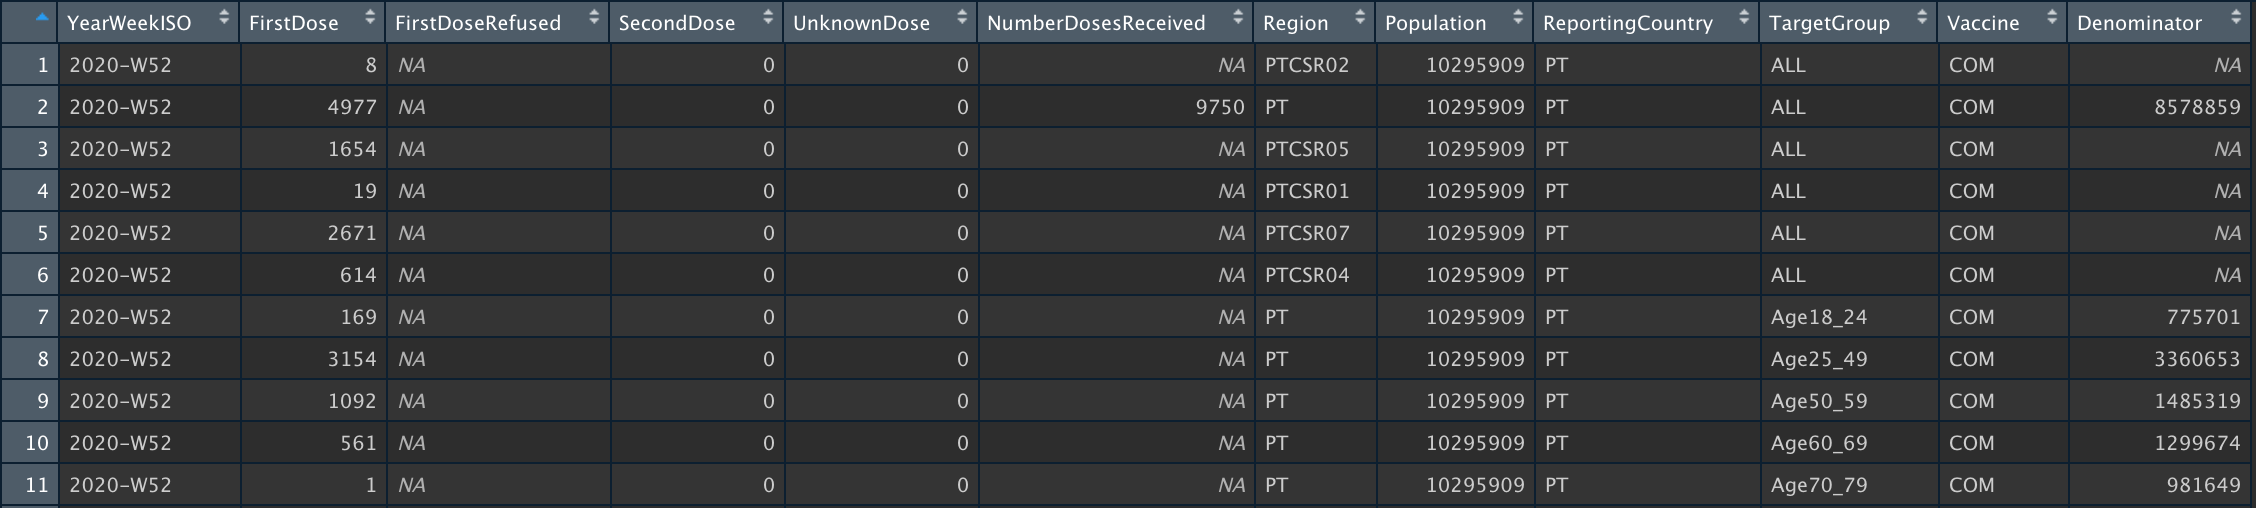
\includegraphics[width=15cm]{images/dataset.png} 

\caption{Excerpt from the dataset }
\label{figura:qualquernome}
\end{figure}





\section{Development}
The R Shiny framework is an RStudio package that makes it incredibly easy to build interactive web applications with R. A Shiny has the benefit of allowing us to create highly effective reports and data visualizations where the user can explore a set of data.

Shiny apps are divided into two parts: 

\begin{itemize}
    \item server.r
    \item ui.r (UI)
    
\end{itemize}
 % se tiver a der merd* corrijam 
 
The ui specification defines:
\begin{itemize}
    \item  Layout functions to configure the visual structure of the html page that will be generated when the application is executed. The fluidPage() function embeds and configures all the necessary and sufficient HTML, CSS and JavaScript code for the application. To create more complex layouts, you need to call layout functions inside fluidPage().
    \item Input control functions that will allow the user to interact with the application. Functions such as sliderInput(), selectInput(), textInput(), numericInput() can be used. All these functions have inputID as their first argument, simple string, with the same restrictions as the object names of R, and unique. This identifier is used to bind the ui to the server.
    If in the ui the inputID = “name”, the server will access it using input?name. The second argument, label, is also important as it contains the text that appears in the application's layout.
    \item Output controls that indicate where to place output with reactive behavior. Examples of output control functions are textOutput(), tableOutput(), among others. As with input control functions, the first argument must be the unique ID. If, for example, in the ui an ID with the name “plot” is defined, on the server the access is output$plot.



 In the server specification, functions that allow calculations to be performed and updated (using reactivity) are implemented. The server controls what data will be through the UI. The server will be where you upload and collate the data and then set your options (ie graphics) using input from the UI.
 
 
 For this purpose, specific rendering functions (render functions) are used. Each render{Type} function produces a specific type of output (for example, renderTable() produces tables, renderText() produces text). Usually these functions are paired with {Type}Output functions (for example renderTable() because it is paired with tableOutput()).


 
 Even though we created two separate files for our application, namely server.r and ui.r , shiny supports single file applications. A single file configuration puts both the server and user interface code in a single app.R file, whereas the multiple file configuration puts them in their own separate files. Functionally, these configurations will produce the same app. The multiple file configuration is generally preferred, especially for larger applications, as it usually makes code easier to manage. For smaller apps, the single file configuration is likely a more efficient way to go.


\subsection{Reactivity in shiny}
Like in other web applications, in Shiny, you express server logic using reactive programming.
\\
The main idea of reactive programming is to specify the dependency graph so that when an input is changed, all related outputs are also updated. 
%for example, we don't need to tell an output to update because due to reactivity, the information is always updated. automatic, making the flow of an application considerably simpler.
\\
Reactivity is what makes applications responsive. Allows the application to update itself instantly whenever the user interacts with the application, requesting any visualization, with updated data.
\\
In Shiny, reactivity creates the illusion that changes to input values automatically flow to the outputs -- graphics, text, and tables that use the input --  and cause them to update. This flow behavior (such as current in a river or electricity) that pushes information from input to output is not real. In fact, in R an expression is only updated when it is executed (lazy evaluation).
\\
So, the idea is: the server re-execute the instructions very frequently, so it knows the input change very quickly, and acts as if it were bound to the input or as if input pushed its new value to the output.
\\
This is the approach that Shiny uses to create reactivity. This is why session R is busy when starting a Shiny application (for example, it is not possible to use the R console when the application is running). The server is using session R to monitor the application and rerun the expressions.
\\
However, Shiny takes this approach a step further, creating an alert system that lets you know exactly what expressions need to be rerun.
\\
Thus, although the server still checks the application at regular intervals (of microseconds), instead of rerunning each expression, it only executes the expressions that the alert system flagged as out of date. If alerts appear, the server executes all expressions that are out of date at the time - this event is called flush and is the key to reactivity as it allows the server to update the application as quickly as possible, appearing to flow instantly from inputs to outputs.
\\
We can see several examples of the use of reactivity in the code of our app. For example, in \verb!UI! (\ref{ui}) and in \verb!server! (\ref{server})
\begin{figure}[h]
\centering % para centralizarmos a figura
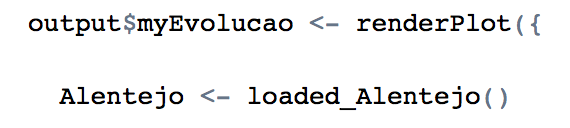
\includegraphics[width=150px]{images/reatividadeUI.png} 
\caption{reactivity:: UI}
\label{ui}
\end{figure}
\begin{figure}[h]
\centering % para centralizarmos a figura
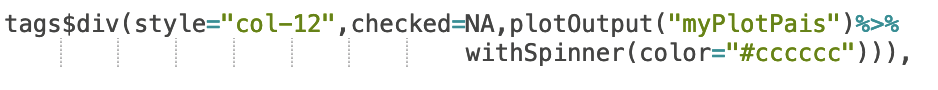
\includegraphics[width=250px]{images/reatividadeSERVER.png} 
\caption{reactivity:: server}
\label{server}
\end{figure}
%In our app we use reactive functions, as it is a way to control which parts of the app are updated, avoiding unnecessary calculations that can slow down your app.

%In our application we use reactive functions as it is a way to control which parts of the application are updated, avoiding unnecessary calculations that can make your application slow.



%\begin{figure}[h]
%\centering % para centralizarmos a figura
%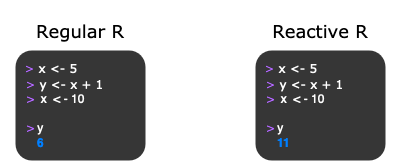
\includegraphics[width=7cm]{images/react.png} 

%\caption{Example of Regular R - Reactive R}
%\label{figura:qualquernome}
%\end{figure}




%For example, in our app //PUT AN EXAMPLE OF OUR APP


\subsection{Render functions}

The main function for generating documents in R Markdown, from the rmarkdown package, is a render ().
The render () function is a wrapper that internally calls knitr :: knit () and later converts the document to .html using Pandoc, which is a document and open source converter.Uma função render que usamos na aplicação foi a renderPlot().

To display the graphics in our application we use the renderPlot () tool. RenderPlot is a reactive function that can take input data from the ui.R script and feed it into the server.R script. It then actively updates the information within its role.



\subsection{Data visualization}
Data visualization through maps, tables or graphs allows contextualizing and understanding information in a natural and efficient way.


R has libraries that allow you to play high-quality graphics. In this work, the ggplot2 package was essentially used, whose methods are based on its own grammar, and where the graphical representations are obtained through the (organized) superposition of several levels that are stacked on top of each other, allowing great flexibility in the construction of the graphs (Hadley Wickham, 2005).


Levels, or layers, consist of data (data.frame format), aesthetic attributes (data mapping definition), geometric objects (visual elements), facets (facets()) functions that allow the execution of multiple graphics related to segments of data defined by factors), statistical transformations, coordinates (space where data is represented) and theme (theme(), functions allow changing individual components of a theme).

\subsection{Application format}





\section{Implementation}
\subsection{Depois ver mais cenas}
\section{Results}
\subsection{Publication}
\subsection{Versatility}

\chapter{Conclusion}


\bibliographystyle{plain}
\begin{thebibliography}{10}


\bibitem{R-project website} \textit{\href{https://www.r-project.org/about.html}{https://www.r-project.org/about.html}} , \textbf{About/R-Project website}

\bibitem{shiny}\textit{\href{https://shiny.rstudio.com/l}{https://shiny.rstudio.com}} , \textbf{Shiny website
}
\bibitem{SARS-CoV-2}\textit{\href{https://apps.who.int/iris/bitstream/handle/10665/332197/WHO-2019-nCoV-FAQ-Virus_origin-2020.1-eng.pdf}{https://apps.who.int/.../origin-2020.1-eng.pdf}} ,\textbf{ Origin of SARS-CoV-2 - \ac{WHO}}

\bibitem{EU}\textit{\href{https://ec.europa.eu/info/live-work-travel-eu/coronavirus-response/public-health/eu-vaccines-strategy_pt}{https://ec.europa.eu/info/live-work-travel-eu/coronavirus-response/public-health/eu-vaccines-strategy_pt}} , \textbf{EU vaccine strategy} 

\bibitem{reuters}\textit{\href{https://graphics.reuters.com/world-coronavirus-tracker-and-maps/vaccination-rollout-and-access/}{https://graphics.reuters.com/world-coronavirus-tracker-and-maps/vaccination-rollout-and-access/}}, \textbf{Covid-19 vaccination tracker, Reuters} 


\bibitem{pubINE}\textit{\href{https://www.ine.pt/xurl/pub/71882686}{https://www.ine.pt/xurl/pub/71882686}}, \textbf{Instituto Nacional de Estatística - Estatísticas Demográficas : 2019. Lisboa : INE, 2020.} 


\bibitem{trab}\textit{\href{https://ec.europa.eu/eures/main.jsp?acro=lmi&lang=pt&countryId=PT&catId=57&parentId=0}{https://ec.europa.eu/eures/main.jsp?acro=lmi&lang=pt&countryId=PT&catId=57&parentId=0}}, \textbf{Labor Market Information - European Commission} 


\bibitem{dataDownload}\textit{\href{https://vaccinetracker.ecdc.europa.eu/public/extensions/COVID-19/vaccine-tracker.html#notes-tab}} , \textbf{General Vaccine information - European Centre for Disease Prevention and Control } 

\end{thebibliography}




